\section{Introduction}

Phenology, the timing of seasonal biological phenomena, is a key aspect of plant and animal life.
It defines the timing and duration of growth and reproduction and thereby determines the ability to capture seasonally variable resources \citep{chuine2017process}.
Phenological analyses often focus on the timing of particular events, such as the dates of peak caterpillar abundance \citep{shutt2019spatial}.
However, for many biological phenomena exact dates of particular events are more difficult to observe than the state of the system itself.
For example, repeated but sparse survey visits may record whether a plant is in bud, flowering, or setting fruit, but not the exact dates when each of those stages was reached.
Such observations can be used to categorize an organism's state into discrete classes which usually follow natural ordering, e.g.\ from least to most developed. 
The resulting data can be described using ordinal regression models \cite{mccullagh1980regression,agresti2010analysis} which then allow inferences about phenological progression.

I here replicate a number of ordinal regression models that were employed by \citet{dennis1986stochastic} and \citet{candy1991modeling} to describe insect phenology. 

\section{Data}
\label{sec:data}
The models replicated in this study are fitted to a data set on the phenology of the western spruce budworm \emph{Choristoneura freemani} (Lepidoptera: Tortricidae), a defoliating moth that is widespread in western North America \citep{brookes1987western}.
This data set was originally published in \citep{dennis1986stochastic} and is a subset of a larger budworm survey data set analysed in \citep{kemp1986stochastic}. 
The data consist of 12 sampling occasions at which counts of individual budworms in each of seven development stages (five larval instars, pupae, and adults) were recorded. 
The only available covariate is a measure of seasonal progression, the accumulated degree days calculated using a threshold of 5.5°C. 
\citet{candy1991modeling} noted an inconsistency in these data, namely that the reported total number of individuals did not correspond to the sum across the seven development stages for two of the sampling occasions. 
I therefore use the data set as it was republished in \citep{candy1990biology}, where numbers in each stage have been assumed correct and the totals for each sampling occasion were adjusted accordingly.

\begin{table}[tbp]
  \small
    \centering
    \caption{The data used in this replication are counts of western spruce budworm \emph{Choristoneura freemani} across seven developmental stages on 12 sampling occasions, as published in \citep{candy1990biology}.}
  
\begin{tabular}{rrrrrrrr}
\toprule
Degree Days & Stage 1 & Stage 2 & Stage 3 & Stage 4 & Stage 5 & Stage 6 & Stage 7\\
\midrule
58 & 16 & 0 & 0 & 0 & 0 & 0 & 0\\
82 & 10 & 0 & 0 & 0 & 0 & 0 & 0\\
107 & 23 & 7 & 0 & 0 & 0 & 0 & 0\\
155 & 3 & 44 & 0 & 0 & 0 & 0 & 0\\
\addlinespace
237 & 0 & 6 & 45 & 13 & 0 & 0 & 0\\
307 & 0 & 2 & 9 & 48 & 15 & 0 & 0\\
342 & 0 & 0 & 1 & 34 & 37 & 0 & 0\\
388 & 0 & 0 & 1 & 10 & 87 & 5 & 0\\
\addlinespace
442 & 0 & 0 & 0 & 7 & 53 & 21 & 0\\
518 & 0 & 0 & 0 & 0 & 10 & 65 & 1\\
609 & 0 & 0 & 0 & 0 & 0 & 14 & 26\\
685 & 0 & 0 & 0 & 0 & 0 & 0 & 42\\
\bottomrule
\end{tabular}
  \label{tab:tab0}
\end{table}

\section{Methods}
The statistical models replicated here are different types of ordinal regression models~\citep{agresti2010analysis}, all with the aim of predicting the proportion of an insect population in a particular development stage at any given time. 
In particular, they represent three different parameterisations of the so-called cumulative model and one version of the so-called sequential model. 
A summary of the theory underlying these models and their derivation is provided in \citep{burkner2019ordinal}.

Both model types assume that the development of an insect follows an unobservable stochastic process $S(t)$ made up of accumulated increments of development over time~$t$. 
As $S(t)$ increases, the insect passes through successive stages $j=1,\dots,r$, delimited by $r-1$ moults, with the $j$th moult occurring when the development threshold $a_j$ is reached:

\begin{alignat*}{3}
  \mathrm{stage}\,1&:\qquad {}&   S(t) & \leq a_1 \\
  \mathrm{stage}\,2&:\qquad  a_1&< S(t) & \leq a_2 \\
  \vdots & &\vdots \\
  \mathrm{stage}\,r-1&:\qquad  a_{r-2}&< S(t) & \leq a_{r-1} \\
  \mathrm{stage}\,r&:\qquad  a_{r-1}&< S(t) 
\end{alignat*}

The $a_j$ values are typically unknown and their estimation from observed data was the goal of the orginal studies~\citep{dennis1986stochastic,candy1991modeling}.

\subsection{Cumulative model with constant variance }
\label{sec:const_var_cm}
The ordinal regression model of~\citep{candy1991modeling} is specified in terms of the cumulative number of individuals  $m_{ij}=\sum_{k=1}^jn_{ik}$ observed in stages 1 to $j$ on a sampling occasion $i$. 
\begin{alignat}{1}
\mathbf{E}(m_{ij})&=N_iPr(S(t) < \alpha_j), \qquad j = 1,\dots ,r\\
&=N_iG(\alpha_j + \beta z_i)
\end{alignat}
where $G$ is the cumulative probability density function of $S(t)$, $\alpha_j$ are ordered thresholds or cut-point parameters, $\beta$ is a vector of regression parameters and $z_i$ is a vector of predictor variables.
If the probability of an individual being in stage $j$ or earlier at time $t_i$ is 

$$\mu_{ij} = \mathbf{E}(m_{ij})/N_i$$

 one can interpret $G^{-1}$ as the link function of a generalised linear model (GLM) with the linear predictor 

$$\eta_{ij}=\alpha+\beta z_i$$

This ordinal regression model is commonly known as the cumulative model~\citep{burkner2019ordinal}, and is applied to the budworm data in \citep{candy1991modeling} using the logit and complementary log-log (cloglog) link functions. 
In both cases the parameterisation results in a constant variance for $S(t)$.
For the purpose of parameter estimation \citet{candy1991modeling} re-expressed the model in terms of stage-specific counts $n_{ij}$  
\begin{equation}
\mathbf{E}(n_{ij})=N_i\{G(\alpha_j + \beta z_i) - G(\alpha_{j-1} + \beta z_i)\}
\label{eq:candy_cm_count_form}
\end{equation}
and fits it using a Poisson likelihood \citep{thompson1981composite}. 
No code or initial values for the likelihood optimisation are provided for this estimation procedure in the original paper.   
I therefore created an R version of the estimation procedure which directly optimizes a Poisson log-likelihood for Equation~\ref{eq:candy_cm_count_form} using the BFGS method in the \verb+optim+ function and a parameter scaling value of 0.01 for $\beta$ relative to the cut-point parameters..
Initial values for the optimisation were determined using a random search across plausible start values (see Appendix~\ref{sec:appendix}).
 The cumulative model is implemented in various R packages, including in the \verb+vglm+ function in \verb+VGAM+ \citep{VGAM} and the \verb+clm+ function in \verb+ordinal+ \cite{ordinal} and for comparison I also attempted to fit the models using these functions with their default settings.

\subsection{Cumulative model with proportional variance}
\citet{dennis1986stochastic} used a different parameterisation of the ordinal model with a logit link, i.e. assuming a logistic distribution for $S(t)$, such that the probability that an insect's development at time $t$ has not exceeded $s$ amounts to 
\begin{equation}
Pr(S(t) \leq s) = \left\{ 1 + \exp\left[-\left(\frac{s-t}{\sqrt{b^2t}}\right)\right]\right\}^{-1}
\label{eqn:cumpropcdf}
\end{equation}
where $b^2$ is a positive constant. 
The cumulative distribution function in Eqn.~\ref{eqn:cumpropcdf} corresponds to a logistic distribution with a mean of $t$ and a variance which increases proportional to the mean as $(\pi^2/3)b^2t$.
At any fixed time $t$ the thresholds $a_j$ segment the probability distribution function into $r$ parts and the area under the curve between $a_{j-1}$ and $a_j$ gives the probability that the insect will be in stage $j$ at time $t$.

This modelling approach is applied to data consisting of samples~$i$ that record the number of insects $x_{ij}$ in stage $j$ at times $t_1, t_2, \dots, t_q$ and the $x_{ij}$ are assumed to be random samples from a multinomial distribution with corresponding multinomial probabilities~$p_{ij}$

\begin{align}
p_{ij} & = Pr(a_{j-1} < S(t_i) \leq a_{j})\\
& =  \left\{ 1 + \exp\left[-\left(\frac{a_j-t_i}{\sqrt{b^2t_i}}\right)\right]\right\}^{-1} - \left\{ 1 + \exp\left[-\left(\frac{a_{j-1}-t_i}{\sqrt{b^2t_i}}\right)\right]\right\}^{-1}\label{eq:dennis_cm}
\end{align}

To fulfill the constraint that $\sum_{j=1}^r p_{ij}= 1$, it is further assumed that $a_0 = -\infty$ and $a_r = +\infty$.
The model has $r$ unknown parameters $a_1, \dots, a_{r-1}$ and $b^2$ which can be found by maximising the corresponding log-likelihood function
\begin{equation}
\mathcal{\ell} = \log C + \sum_{j=1}^r \sum_{i=1}^q x_{ij} \log p_{ij}
\label{eq:dennis_loglik}
\end{equation}
where $C$ is a combinatorial constant that is independent of the parameter values.

\citet{dennis1986stochastic} provided SAS code and initial values to estimate the parameters under this likelihood using an iteratively reweighted non-linear least squares approach based on \verb+PROC NLIN+. 
This was updated to run in a contemporary version of SAS (SAS 9.4) and is provided in the article code repository. 
However, since SAS is a proprietary software package, I implemented two R versions of the estimation procedure which both directly optimize the log-likelihood (\ref{eq:dennis_loglik}) using the L-BFGS-B optimisation routine \citep{byrd1995limited} in the R \verb+optim+ function. The first implementation is a direct translation of the SAS code which uses a literal implementation of the logistic cumulative distribution function and employs a lower parameter bound of 0 and initial values provided in \citep{dennis1986stochastic} for the estimation. The second implementation makes use of the R function \verb+stats::plogis+ to implement the logistic CDF and employs a lower parameter bound of the machine precision (i.e.\ \verb+.Machine$double.xmin+) and the same initial values as above. Both routines used a parameter scaling value of 0.01 for $b^2$ relative to the cut-point parameters

\citet{candy1991modeling} re-expressed the proportional variance model (Eqn.~\ref{eq:dennis_cm}) to match the form of Eqn.~\ref{eq:candy_cm_count_form}, which results in the following re\-para\-meter\-isation $\alpha_j = a_j/b$, $\beta = -1/b$, and $z_i = \sqrt{t_i}$, and uses the Poisson likelihood approach described in section~\ref{sec:const_var_cm} for parameter estimation. 
A set of example macros for the software package \verb+GLIM+ \citep{aitkin1989statistical} is provided in an earlier manuscript by the same author \citep{candy1990biology}. GLIM is no longer actively developed or distributed, but initial values from the GLIM code were used in the estimation with the BFGS method of R \verb+optim+ and a parameter scaling value of 0.01 for $\beta$ relative to the cut-point parameters.

\subsection{Sequential model}
A different class of ordinal regression model can be derived by treating the observations as the result of a strictly ordered counting process, i.e.\ to achieve a stage $j$, all lower stages $1,\dots,j-1$ have to be achieved first. 
The general form of this model is known as the sequential model, and rather than assuming a single latent process $S(t)$ as in the cumulative model there is a latent continuous variable $S_j$ for each category $j$~\citep{burkner2019ordinal}. 
Analogous to the cumulative model it can be framed as a GLM 

\begin{equation}
S_j = \eta + \epsilon_j
\end{equation}

with a linear predictor $\eta$ and an error term $\epsilon_j$ which has mean zero and is distributed following some distribution $G$. 
This leads to a model of the form 

\begin{equation}
Pr(S = a_j|S \geq a_j, \eta) = G(a_j - \eta)
\end{equation}

When $G$ is the logistic distribution this model is also known as the continuation ratio model~\citep{fienberg1980analysis,burkner2019ordinal}. 
Confusingly, there are two common versions of the model in the literature both using this name. 
The one outlined above describing the probability of the sequential process \emph{stopping} at stage $j$, and the other describing the probability of the process \emph{continuing} beyond stage $j$, i.e. 

$Pr(S > a_j | S \geq a_j, \eta)$ \citep{burkner2019ordinal,VGAM}. 

The paper replicated here \citep{candy1991modeling} used the stopping parameterisation.
In their notation the expected value for the stage-specific counts $n_{ij}$ is
\begin{alignat}{3}
\mathbf{E}(n_{ij})&=N_i G(\beta_{01} + \beta_{11}t_i), &j&=1 \label{eq:candy_sm_counts}\\
&=N^*_{ij} G(\beta_{0j} + \beta_{1j}t_i), \qquad &j&=2,\dots,r-1 \nonumber
\end{alignat}
with 
\begin{equation}
N^*_{ij}=\left(N_i - \sum_{k=1}^{j-1}n_{ik}\right) \label{eq:n_star}
\end{equation}
and conditional probabilities 
\begin{equation}
p^*_{ij} =  G(\beta_{0j} + \beta_{1j}t_i), \qquad j=1,\dots,r-1
\end{equation}

\citet{candy1991modeling} uses GLM estimation routines in \verb+GLIM+ to fit the $r-1$ models defined in Eqn.~\ref{eq:candy_sm_counts} assuming the $n_{ij}$ are binomially distributed conditional on $N_i$ for stage 1 and conditional on $N^*_{ij}$ for stages $2,\dots,r-1$. 
No code is provided for this estimation procedure in the original paper, but the model is straightforward to implement using the \verb+glm+ function in R with a model formula of the form 
$$\verb!cbind(count,total - N_star) ~ stage + stage:time - 1!$$
where the variable \verb+count+ represents the $n_{ij}$, \verb+N_star+ represents $N_i$ for $j=1$ and $N^*_{ij}$ for all other observations, \verb+stage+ is a factor variable encoding $j$ and \verb+time+ are the $t_i$. The sequential model with stopping parameterisation is also implemented in \verb+VGAM::vglm+ \citep{VGAM} and for comparison I attempted to fit the model using this function with its default settings.


\section{Results}



\begin{table}[tbp]
  \small
    \centering
    \caption{Parameter estimates for the cumulative model with constant variance (Eqn.~\ref{eq:candy_cm_count_form}). 
    This table replicates results presented in the first two rows of Table~2 of \citep{candy1991modeling}. 
    Note that \texttt{ordinal::clm} uses a parameterisation $\alpha_j - \beta z_i$ for the linear predictor yielding a parameter estimate for $\beta$ with the opposite sign than the other methods. 
    The cloglog link model failed to fit using \texttt{VGAM::vglm}.}
  
\begin{tabular}{ccccccccc}
\toprule
Method & $\alpha_1$ & $\alpha_2$ & $\alpha_3$ & $\alpha_4$ & $\alpha_5$ & $\alpha_6$ & $\beta$ & Link\\
\midrule
Original \citep{candy1991modeling} & 5.49 & 9.39 & 12.23 & 15.70 & 21.26 & 27.25 & -0.0457 & logit\\
R \verb+optim+ & 5.47 & 9.36 & 12.21 & 15.67 & 21.22 & 27.19 & -0.0456 & logit\\
R \verb+clm+ & 5.47 & 9.36 & 12.21 & 15.67 & 21.22 & 27.19 & 0.0456 & logit\\
R \verb+vglm+ & 5.47 & 9.36 & 12.21 & 15.67 & 21.22 & 27.19 & -0.0456 & logit\\
\addlinespace
Original \citep{candy1991modeling} & 3.32 & 5.85 & 7.72 & 10.03 & 13.46 & 17.52 & -0.0307 & cloglog\\
R \verb+optim+ & 3.32 & 5.85 & 7.71 & 10.02 & 13.46 & 17.52 & -0.0307 & cloglog\\
R \verb+clm+ & 3.32 & 5.85 & 7.71 & 10.02 & 13.46 & 17.52 & 0.0307 & cloglog\\
R \verb+vglm+ & NA & NA & NA & NA & NA & NA & NA & cloglog\\
\bottomrule
\end{tabular}
  \label{tab:tab1}
\end{table}

\begin{table}[tbp]
  \small
    \centering
    \caption{Parameter estimates for the cumulative logit model with proportional variance. 
    This table replicates results presented in the first row of Table~1 of  \citep{kemp1986stochastic} and the last row of Table~2 of \citep{candy1991modeling}.}
  
\begin{tabular}{ccccccccc}
\toprule
Method & $a_1$ & $a_2$ & $a_3$ & $a_4$ & $a_5$ & $a_6$ & $b^2$ & Eqn.\\
\midrule
Original \citep{kemp1986stochastic} & 121.080 & 204.360 & 264.410 & 342.473 & 465.620 & 599.570 & 1.559 & \ref{eq:dennis_cm}\\
SAS \verb+NLIN+ & 120.000 & 204.700 & 264.600 & 341.300 & 464.500 & 595.700 & 1.412 & \ref{eq:dennis_cm}\\
R \verb+optim+ & 120.033 & 204.659 & 264.586 & 341.285 & 464.480 & 595.690 & 1.412 & \ref{eq:dennis_cm}\\
\midrule $\alpha_1$ & $\alpha_2$ & $\alpha_3$ & $\alpha_4$ & $\alpha_5$ & $\alpha_6$ & $\beta$ & Method & Eqn. \\ \midrule
Original \citep{candy1991modeling} & 101.000 & 172.200 & 222.700 & 287.200 & 390.900 & 501.300 & -0.842 & \ref{eq:candy_cm_count_form}\\
R \verb+optim+ & 100.989 & 172.181 & 222.598 & 287.134 & 390.771 & 501.157 & -0.841 & \ref{eq:candy_cm_count_form}\\
\bottomrule
\end{tabular}
  \label{tab:tab2}
\end{table}


\subsection{Cumulative model with constant variance}
Parameters were estimated using a direct optimisation of the Poisson likelihood for Eqn.~\ref{eq:candy_cm_count_form}, as well as with the R functions \verb+VGAM::vglm+ and \verb+ordinal::clm+. 
The cloglog link model failed due to numerical errors when using the \verb+vglm+ function. 
Parameter estimates were close to those of the original study for all three methods employed (Table~\ref{tab:tab1}). Parameter estimates were generally insensitive to the choice of starting values once the optimisation function was provided with appropriate parameter scaling values for the optimisation routine (see Appendix).

\subsection{Cumulative model with proportional variance}
The original SAS code provided in \citep{dennis1986stochastic} required minimal updates to run in a contemporary version of SAS (SAS 9.4). 
Translating the model code to R was straightforward once I took the decision to implement a direct minimisation of the negative log likelihood with \verb+optim+.  

Parameter estimates from SAS \verb+NLIN+ and both R \verb+optim+ implementations (Table~\ref{tab:tab2}) were virtually identical, but differed slightly from the parameter estimates presented in \citep{kemp1986stochastic}, which was assumed to be the original source for the parameter estimates, as no parameter estimates were presented in \citep{dennis1986stochastic}. 
The observed differences in estimates were $<1$\% for the cut-point parameters $\alpha_i$, but c. 9\% for $\beta$.

Based on these three sets of parameter estimates it was also possible to redraw two figures from \citep{dennis1986stochastic}. 
Figure~\ref{fig:fig1} and~\ref{fig:fig2}, respectively, show that despite the observed parameter differences  there is an overall good agreement between the original results and the replication.

\begin{figure}[p]
  \centering
  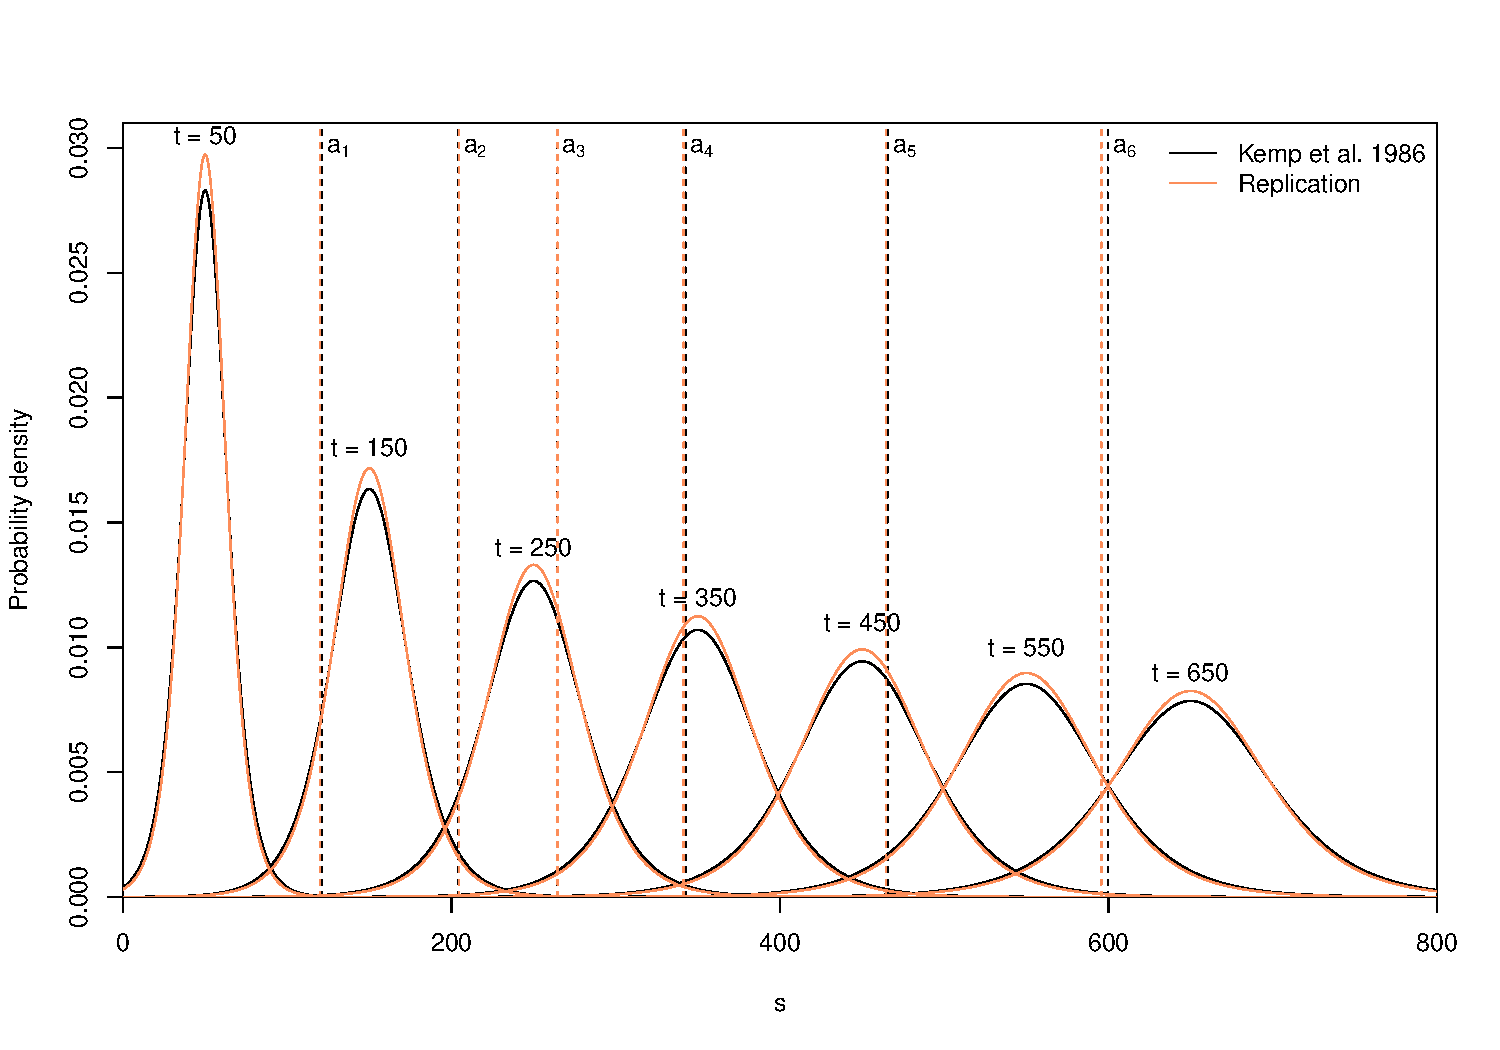
\includegraphics[width=\textwidth]{../figures/fig1_dennis_fig2.pdf}
  \caption{Logistic PDF of the cumulative model with proportional variance (Equation~\ref{eq:dennis_cm}) plotted for fixed values of~$t$. 
  Area under the PDF between $a_{j-1}$ and $a_j$ gives the expected proportion of insects in stage $j$ at time $t$. 
  The graph is based on the estimates in Table 1 of \citep{kemp1986stochastic} (black lines) and the estimates from the replication using the R \texttt{optim} implementation (red lines). 
  This figure replicates Figure 2 in \citep{dennis1986stochastic}.}
  \label{fig:fig1}
\end{figure}


\begin{figure}[p]
  \centering
  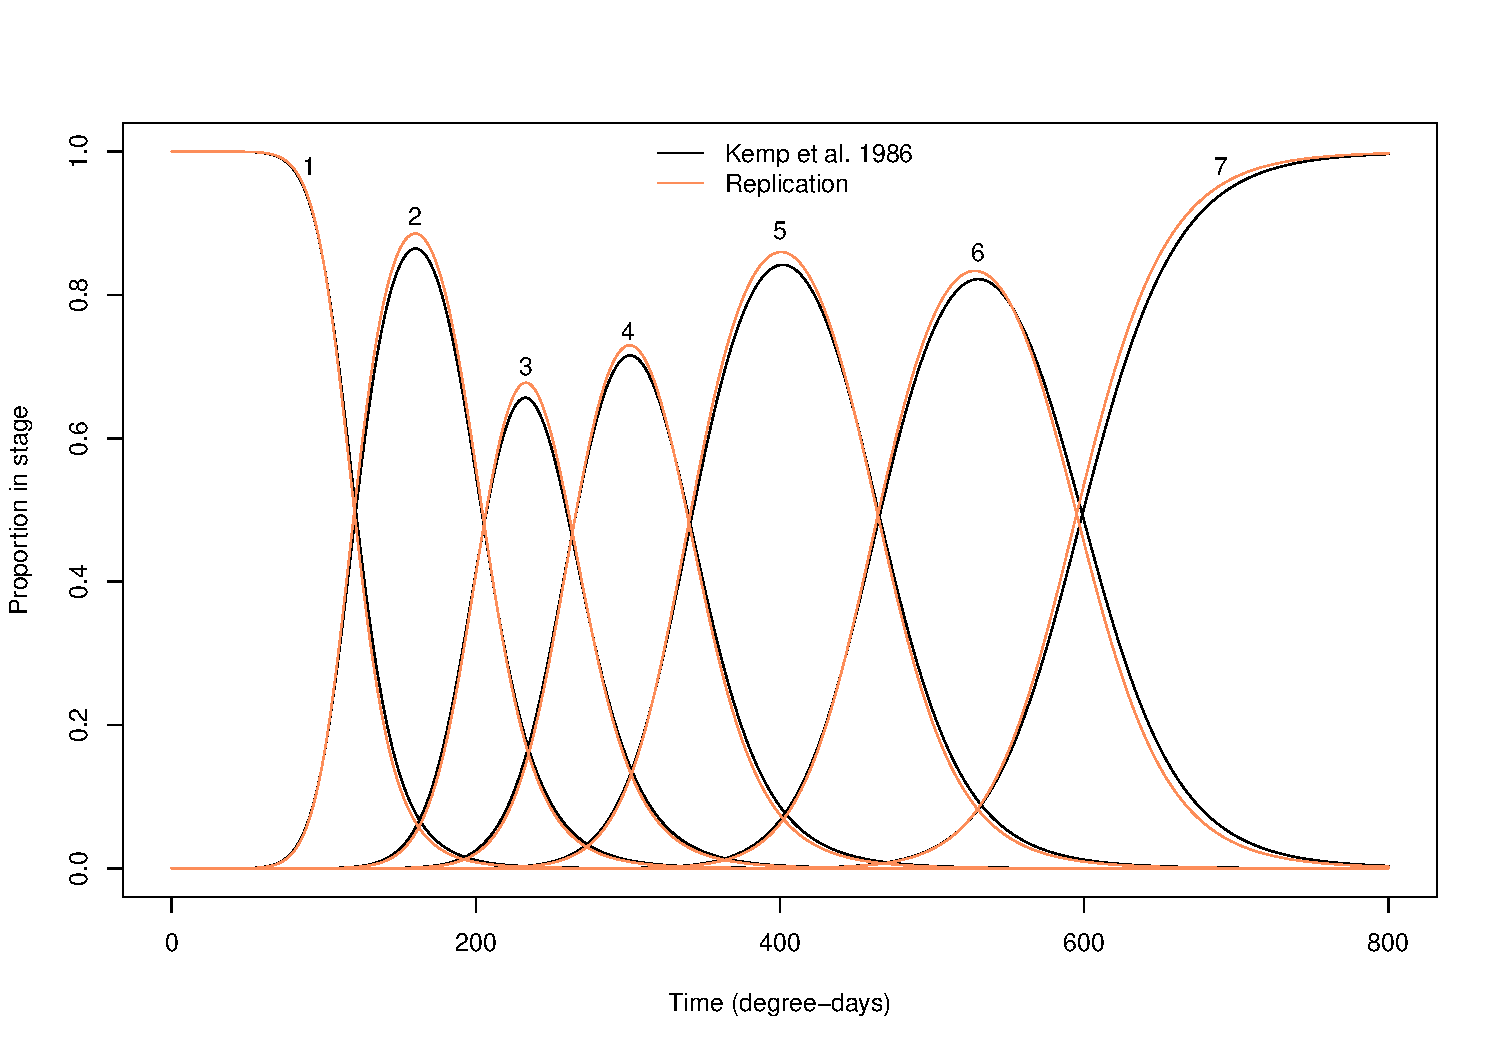
\includegraphics[width=\textwidth]{../figures/fig2_dennis_fig3.pdf}
  \caption{Proportion of insects expected in stages 1-7 under the cumulative logit model with proportional variance (Equation~\ref{eq:dennis_cm}) plotted as functions of time $t$.
   Values of $a_j$ and $b^2$ used in the graph are the estimates given in Table 1 of \citep{kemp1986stochastic} (black lines) and the estimates from the replication using the R \texttt{optim} implementation (red lines). 
   This figure replicates Figure 3 in \citep{dennis1986stochastic}.}
  \label{fig:fig2}
\end{figure} 

\begin{table}[htb]
  \small
    \centering
    \caption{Parameter estimates for the sequential model with stopping ratios (Equation~\ref{eq:candy_sm_counts}). 
    This table replicates results presented in Table~3 of \citep{candy1991modeling}. 
    The cloglog link model failed to fit using \texttt{VGAM::vglm}.}
  
\begin{tabular}{lrrrrrrll}
\toprule
Parameter & $\beta_{\_1}$ & $\beta_{\_2}$ & $\beta_{\_3}$ & $\beta_{\_4}$ & $\beta_{\_5}$ & $\beta_{\_6}$ & Link & Method\\
\midrule
$\beta_{0j}$ & 10.410 & 12.960 & 12.020 & 11.160 & 17.700 & 33.730 & logit & Original \citep{candy1991modeling}\\
$\beta_{0j}$ & 10.410 & 12.959 & 12.020 & 11.165 & 17.698 & 33.726 & logit & R \verb+vglm+\\
$\beta_{1j}$ & -0.085 & -0.062 & -0.046 & -0.033 & -0.038 & -0.056 & logit & Original \citep{candy1991modeling}\\
$\beta_{1j}$ & -0.085 & -0.062 & -0.046 & -0.033 & -0.038 & -0.056 & logit & R \verb+vglm+\\
\addlinespace
$\beta_{0j}$ & 7.350 & 8.530 & 9.120 & 8.440 & 10.090 & 16.300 & cloglog & Original \citep{candy1991modeling}\\
$\beta_{0j}$ & NA & NA & NA & NA & NA & NA & cloglog & R \verb+vglm+\\
$\beta_{1j}$ & -0.065 & -0.044 & -0.037 & -0.026 & -0.023 & -0.029 & cloglog & Original \citep{candy1991modeling}\\
$\beta_{1j}$ & NA & NA & NA & NA & NA & NA & cloglog & R \verb+vglm+\\
\bottomrule
\end{tabular}
  \label{tab:tab3}
\end{table}

\subsection{Sequential model}
\label{sec:sm-results}
Parameters were estimated using the R \verb+glm+ function and \verb+VGAM::vglm+. 
The GLM formulation of the model fitted with R \verb+glm+ produced a warning that fitted probabilities numerically 0 or 1 occurred. 
Likely due to related reasons, the cloglog link model failed due to numerical errors when using the \verb+vglm+ function. 
Parameter estimates, where obtained, were identical to the original study (Table~\ref{tab:tab3}) within the precision reported in \citep{candy1991modeling}.

\section{Discussion}
Overall the results from both \citep{dennis1986stochastic} and \citep{candy1991modeling} could be replicated closely.
The SAS code provided in \citep{dennis1986stochastic} required only minimal updates to run in a contemporary version of SAS (SAS 9.4) and produced virtually identical estimates to the R re-implementation. 
These estimates, however, differed slightly from the parameter estimates reported in \citep{kemp1986stochastic}. 
Given that the same initial values were used in all implementations, I believe that this disagreement is most likely caused by the inconsistencies in the published data set described in Section~\ref{sec:data}. 
The corrections applied to the data by \citep{candy1991modeling} result in a data set that is internally consistent but likely different to that on which the estimates in \citep{kemp1986stochastic} are based.  

No code was provided in \citep{candy1991modeling}. 
However, the mathematical and verbal descriptions of the models were detailed enough to re-implement the estimation procedures in R. 
GLIM code of the cumulative model with proportional variance was available from an earlier manuscript~\citep{candy1990biology}. 
This allowed me to use the same initial values as the original study for this model. 
Initial values for the model with constant variance had to be guessed.
The direct optimisation of the likelihood was reported to be sensitive to the choice of initial values in ~\citep{dennis1986stochastic}. 
Additional simulations (Appendix~\ref{sec:appendix}) showed that convergence failures did occur for some initial values, particularly in the case for the cloglog-link model.
However, the coefficient of variation for estimates derived from a wide range of initial values was very small (<0.01\%) for both the logit and cloglog models, whenenver the model converged succesfully (Table~\ref{tab:tabS2}).

Literal implementations of both the inverse logit and inverse complementary log-log function can suffer from numerical underflow and/or overflow for probabilities close to zero and one, and this may be the key reason for convergence failures observed in the direct optimisation, as well as in the \verb+vglm+ function. 
The case study presented here is based on observations where the population variation in development speed (i.e.\ the transition from class to class) is low compared to the overall speed of seasonal progression.
As a result the early and late development stages of the observed species never occur together, and the observed data are sparse in the sense that many cell counts in Table~\ref{tab:tab0} are zero.
As a consequence the model estimates large effects, which although estimable on the link scale, are indistinguishable from one on the probability scale given the limitations of floating point representations.
This is the underlying reason for the warnings produced by the \verb+glm+ function when fitting the sequential model.
The GLIM code for the cumulative model from \citep{candy1990biology} uses multiple thresholding steps during the calculation of the linear predictor to mitigate against this, whereas the R implementation of the corresponding model makes use of a single thresholding step in the inverse link function (\verb+gtools::inv.logit+~\citep{gtools} or \verb+stats::plogis+ and \verb+VGAM::clogloglink+, respectively). 
Differences in parameter estimates between a literal implementation of the logit link and  \verb+stats::plogis+ for the cumulative model with proportional variance (Table~\ref{tab:tab3}) were less than 0.01\%, however, in the case of the constant variance model the complementary log-log link model proved to be numerically less stable than the corresponding logit-link model (Figure~\ref{fig:figS1}). 
This is perhaps unsurprising as the cloglog function has a steeper slope as it approaches one compared to the logit function, so values numerically close to one are attained earlier.
Given the sparsity of the data set and the resulting large estimated effect sizes this likely contributed to the failure to fit either of the cloglog-link models using the \verb+VGAM::vglm+ function.
The behaviour was reported to the maintainer of the \verb+VGAM+package, and initial troubleshooting of the\verb+VGAM+ code resolved some instabilities for the fitting of the cumulative model.
These updates are now available in the pre-release version of \verb+VGAM+\footnote{https://www.stat.auckland.ac.nz/~yee/VGAM/prerelease/index.html}.
However, other instabilities remain. 
The cumulative model using the updated \verb+VGAM+ code converges far from the optimum identified by the other methods and a fix for the error affecting the sequential model are yet to be implemented.

\section*{Acknowledgements}
I am grateful to Juniper Simonis and Andrew MacDonald for constructive reviews of an earlier version of this manuscript, and to Thomas Yee for investigating numerical errors in the \verb+VGAM+ package.

\afterpage{\clearpage}
